\documentclass[]{article}

\usepackage[portuguese]{babel}
\usepackage[utf8]{inputenc}
\usepackage{indentfirst}
\usepackage{listings}
\usepackage{graphicx}
\usepackage{verbatim}
\usepackage{mathptmx}
\usepackage[a4paper]{geometry}
\usepackage{color}
\usepackage{amsmath}
\usepackage[section]{placeins}
\usepackage{float}

\definecolor{dkgreen}{rgb}{0,0.6,0}
\definecolor{gray}{rgb}{0.5,0.5,0.5}
\definecolor{mauve}{rgb}{0.58,0,0.82}


\lstset{ %
  language=python,                % the language of the code
  basicstyle=\footnotesize,       % the size of the fonts that are used for the code
  numbers=left,                   % where to put the line-numbers
  numberstyle=\tiny\color{gray},  % the style that is used for the line-numbers
  stepnumber=1,                   % the step between two line-numbers. If it's 1, each line 
                                  % will be numbered
  numbersep=5pt,                  % how far the line-numbers are from the code
  backgroundcolor=\color{white},  % choose the background color. You must add \usepackage{color}
  showspaces=false,               % show spaces adding particular underscores
  showstringspaces=false,         % underline spaces within strings
  showtabs=false,                 % show tabs within strings adding particular underscores
  frame=single,                   % adds a frame around the code
  rulecolor=\color{black},        % if not set, the frame-color may be changed on line-breaks within not-black text (e.g. commens (green here))
  tabsize=4,                      % sets default tabsize to 2 spaces
  captionpos=b,                   % sets the caption-position to bottom
  breaklines=true,                % sets automatic line breaking
  breakatwhitespace=false,        % sets if automatic breaks should only happen at whitespace
  title=\lstname,                 % show the filename of files included with \lstinputlisting;
                                  % also try caption instead of title
  keywordstyle=\color{blue},          % keyword style
  commentstyle=\color{dkgreen},       % comment style
  stringstyle=\color{mauve},         % string literal style
  escapeinside={\%*}{*)},            % if you want to add a comment within your code
  morekeywords={*,...}               % if you want to add more keywords to the set
}

% this is needed for forms and links within the text
\usepackage[hidelinks]{hyperref} 

%IART1718_INT_GE1_3
\title{IART - Relatório Final}
\author{
	André Miguel Ferreira da Cruz (201503776);\\
    Edgar Filipe Amorim Gomes Carneiro (201503784);\\
	João Filipe Lopes de Carvalho (201504875);\\
}

\begin{document}
\setlength{\textwidth}{18cm}
\setlength{\textheight}{22cm}


\begin{titlepage}
  \begin{center}
    \vspace*{1cm}
    
	
      \Huge
      \textbf{Relatório Intercalar}\\
      \vspace{0.5cm}
      \LARGE Redes Neuronais para a identificação de Pulsares

    \vspace{1.5cm}

    
\includegraphics[scale=0.15]{img/feup_logo.png}
    
	\vfill
	
	\Large{Mestrado Integrado em Engenharia Informática e Computação}\\
    \vspace{0.5cm}
	\Large\textbf{IART - Inteligência Artificial}\\
    
    \vspace{0.8cm}
    \large
    Turma 3MIEIC02, Grupo E1\_3 :\\
    André Miguel Ferreira da Cruz - 201503776\\
    Edgar Filipe Amorim Gomes Carneiro - 201503784\\
	João Filipe Lopes de Carvalho - 201504875\\
    \vspace{0.8cm}

    \Large
    Faculdade de Engenharia da Universidade do Porto\\
    Rua Roberto Frias, s/n, 4200-465 Porto, Portugal\\
    
    \vspace{1cm}
    \today

  \end{center}
\end{titlepage}
\newpage

%************************************************************************************
%************************************************************************************

\tableofcontents
\newpage

%************************************************************************************
%************************************************************************************

\section{Objetivo}
\label{sec:intro}
	Este trabalho tem como objetivo a aplicação de Redes Neuronais artificiais na identificação de Pulsares. Neste sentido, começamos por expor e explicitar o tema, com uma pequena introdução à tarefa em questão, e às dificuldades à sua resolução (Secção~\ref{sec:intro}). De seguida, analisamos o \textit{dataset} em uso, descrevendo características e possíveis tendências (\textit{bias}) indesejadas (Secção~\ref{sec:dataset}). No mesmo sentido, explicamos o pré-processamento necessário (Secção~\ref{sec:preprocessamento}), bem como o modelo de aprendizagem a aplicar (Secção~\ref{sec:redes_neuronais}), a sua arquitetura (Secção~\ref{sec:arquitetura}), e as métricas usadas para avaliar adequadamente o desempenho do sistema (Secção~\ref{sec:avaliacao}). De seguida, é detalhado o ambiente de desenvolvimento usado, as ferramentas e bibliotecas a que recorremos, bem como a estrutura da aplicação desenvolvida (Secção~\ref{sec:desenvolvimento}). Finalmente, expomos todo o trabalho efetuado para resolver o problema, e avaliamos minuciosamente os modelos desenvolvidos e os seus resultados (Secção~\ref{sec:experiencias}). Para concluir, enumeramos possíveis melhoramentos para trabalho futuro (Secção~\ref{sec:melhoramentos}), e extraímos conclusões das experiências efetuadas e dos resultados obtidos (Secção~\ref{sec:conclusao}).
	
    Os pulsares são um tipo de estrelas de neutrões raro que, devido ao seu intenso campo magnético, transforma energia cinética (rotacional) em energia eletromagnética. Além disso, o seu campo magnético é suficientemente forte para arrancar partículas da sua superfície (na sua maioria eletrões), que são depois aceleradas na \textit{magnetosfera} e emitidas sob a forma de um feixe estreito e contínuo. Este feixe de radiação, juntamente com a contínua rotação do pulsar, gera um sinal característico, análogo ao de um farol em rotação, de intensidade suficiente para ser detetado a milhões de anos-luz de distância. Desta forma, a deteção de um pulsar corresponde à procura e reconhecimento dos seus sinais periódicos.
    
    Cada pulsar produz um padrão próprio, distinto dos restantes corpos celestes, e que varia ligeiramente entre diferentes pulsares. Assim, podemos detetar um sinal, realizando uma análise de alguns parâmetros, como por exemplo o tempo médio que um pulsar demora a reemitir o seu feixe para a terra. À primeira vista, concluir se um sinal é realmente proveniente de um pulsar pode parecer pouco complexo. No entanto, devido a fortes interferências de frequências de rádio e de sinais ruidosos que dificultam a receção de sinais genuínos, a grande maioria das supostas deteções são falsas.
    
    Devido às dificuldades referidas anteriormente, e ao grande volume de dados em causa (induzido maioritariamente por falsas deteções), esta tarefa torna-se extenuante e dispendiosa para humanos, tornando-a uma muito boa candidata para a aplicação de técnicas de \textit{Machine Learning}.
    Os algoritmos de \textit{machine learning} funcionam através da construção de um modelo a partir de inputs amostrais, com a finalidade de fazer previsões ou decisões orientadas pelos dados e respetivas estatísticas, ao invés de seguir estruturas de decisão estáticas.
    
    Assim sendo, neste trabalho iremos usar algoritmos de aprendizagem supervisionada, nomeadamente redes neuronais artificias, como forma de resolução do problema de classificação apresentado.\\

%************************************************************************************
%************************************************************************************


\section{Especificação}
\label{sec:descricao}
	Esta secção comporta a descrição dos dados usados, a explicitação da etapa de pré-processamento dos dados, bem como uma explicação mais detalhada do modelo de aprendizagem a aplicar. Por fim, é descrito o trabalho efetuado até ao momento, os resultados obtidos, as métricas usadas para a avaliação, bem como futuro trabalho no sentido de melhorar o desempenho do modelo.
    
\subsection{Descrição e análise do dataset.}
\label{sec:dataset}
	Nesta secção, é feita uma análise do \textit{dataset} em uso, especificando o seu conteúdo e determinando as suas características e possíveis tendências (\textit{bias}) indesejadas.
    
	Na base de dados fornecida, cada candidato é caraterizado por oito variáveis continuas e uma classe. As oito variáveis contínuas distinguem-se em dois grupos, sendo  as primeiras quatro referentes a estatísticas relativas ao \textit{folded profile} de um pulsar, e as restantes quatro relativas às características da curva \textit{DM-SNR} (\textit{Delta Modulation with Signal-to-Noise Ratio}). O primeiro grupo consiste num \textit{array} de variáveis contínuas que descrevem uma versão pós-análise do pulsar. E as variáveis do segundo grupo são obtidas através da análise da curva \textit{DM-SNR}. Esta consiste na modulação de um sinal analógico para digital ou o seu reverso. Por sua vez, a classe fornecida como último parâmetro tem um binário, indicando se o candidato era de facto um pulsar ou não. Em relação a cada um dos grupos são obtidas quatro variáveis contínuas: valor médio, desvio padrão, curtose e assimetria.

	A base de dados fornecida contém um total de 17,898 entradas, sendo que destas, 16,259 tratam-se de dados espúrios causados pelo ruído (classe negativa) e as restantes 1,639 tratam-se de dados relativos a sinais de pulsares reais (classe positiva). Para melhor visualização dos dados fornecidos, a Figura~\ref{fig:distribuicoes} apresenta as distribuições das 8 variáveis contínuas de \textit{input}. Essas mesmas distribuições encontram-se pormenorizadas na Figura~\ref{fig:descricao_do_dataset}, sob a forma de tabela.

    \begin{figure}[h]
	\centering
	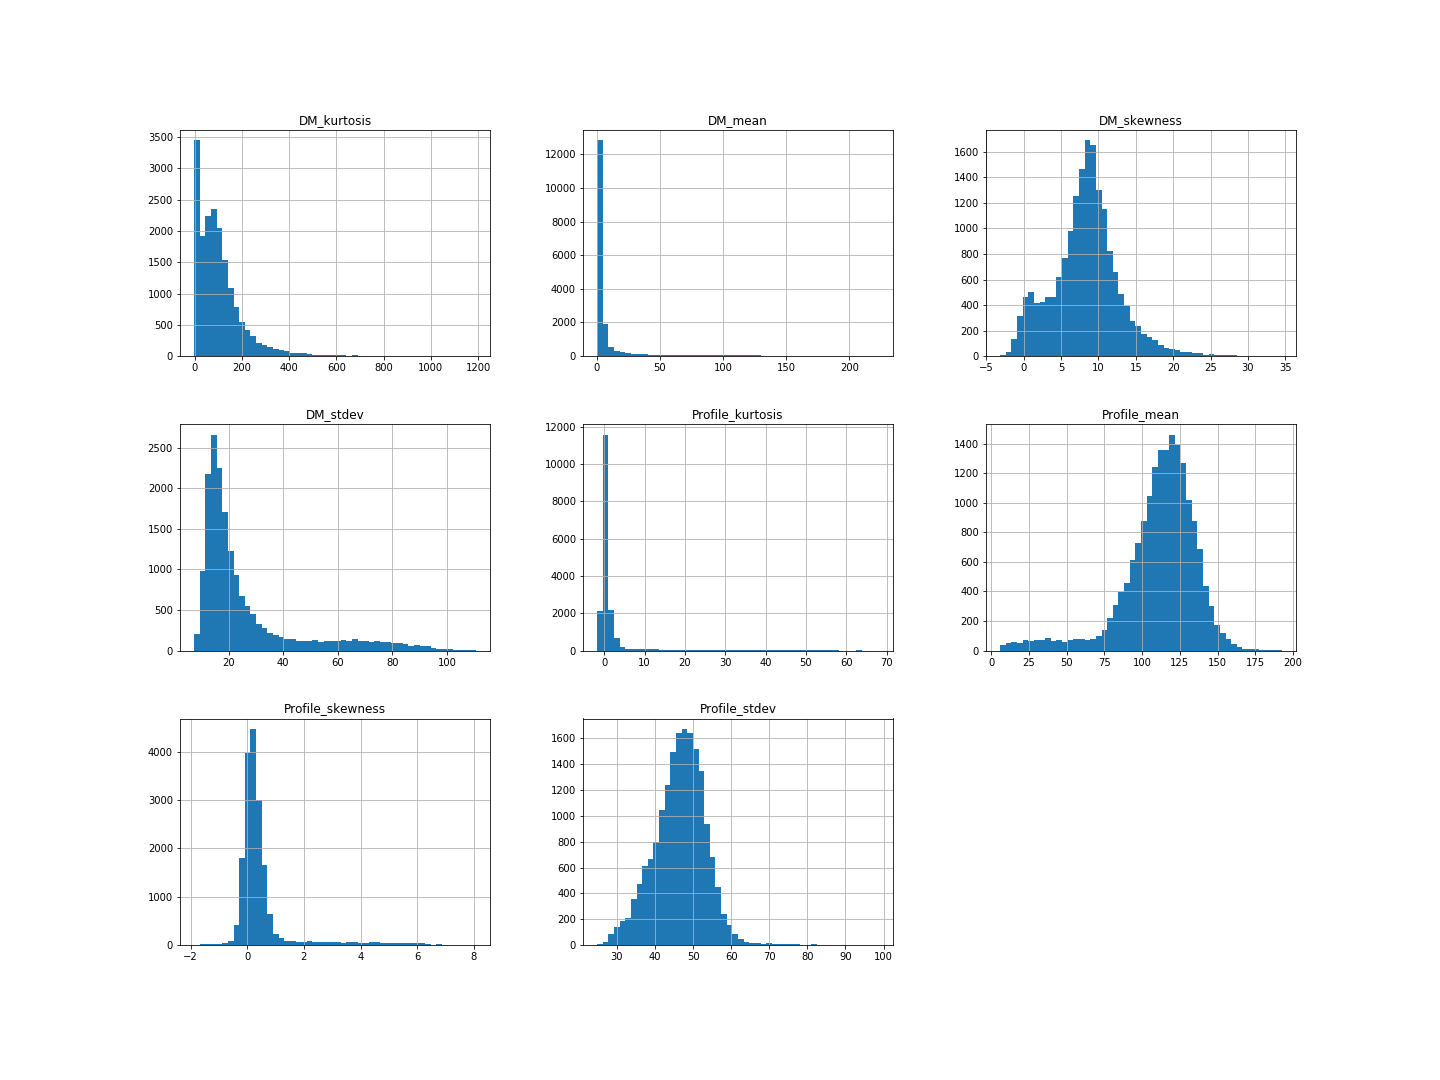
\includegraphics[scale=0.3]{img/distribution.png}
    \caption{Distribuições relativas às 8 variáveis contínuas. Por ordem, da esquerda para a direita, e de cima para baixo, temos: Curtose da curva \textit{DM-SNR}, Média da curva \textit{DM-SNR}, Assimetria da curva \textit{DM-SNR}, Desvio Padrão da curva \textit{DM-SNR}, Curtose do \textit{folded profile}, Média do \textit{folded profile}, Assimetria do \textit{folded profile} e Desvio padrão do \textit{folded profile}.}
    \label{fig:distribuicoes}
    \end{figure}
    
    Assim sendo, para esta tarefa de classificação binária os valores das oito variáveis relativas ao sinal são usados na análise de cada candidato, de forma a determinar se se trata ou não de um pulsar (informação fornecida na 9ª coluna do \textit{dataset}).
    
    \begin{figure}[t]
	\centering
	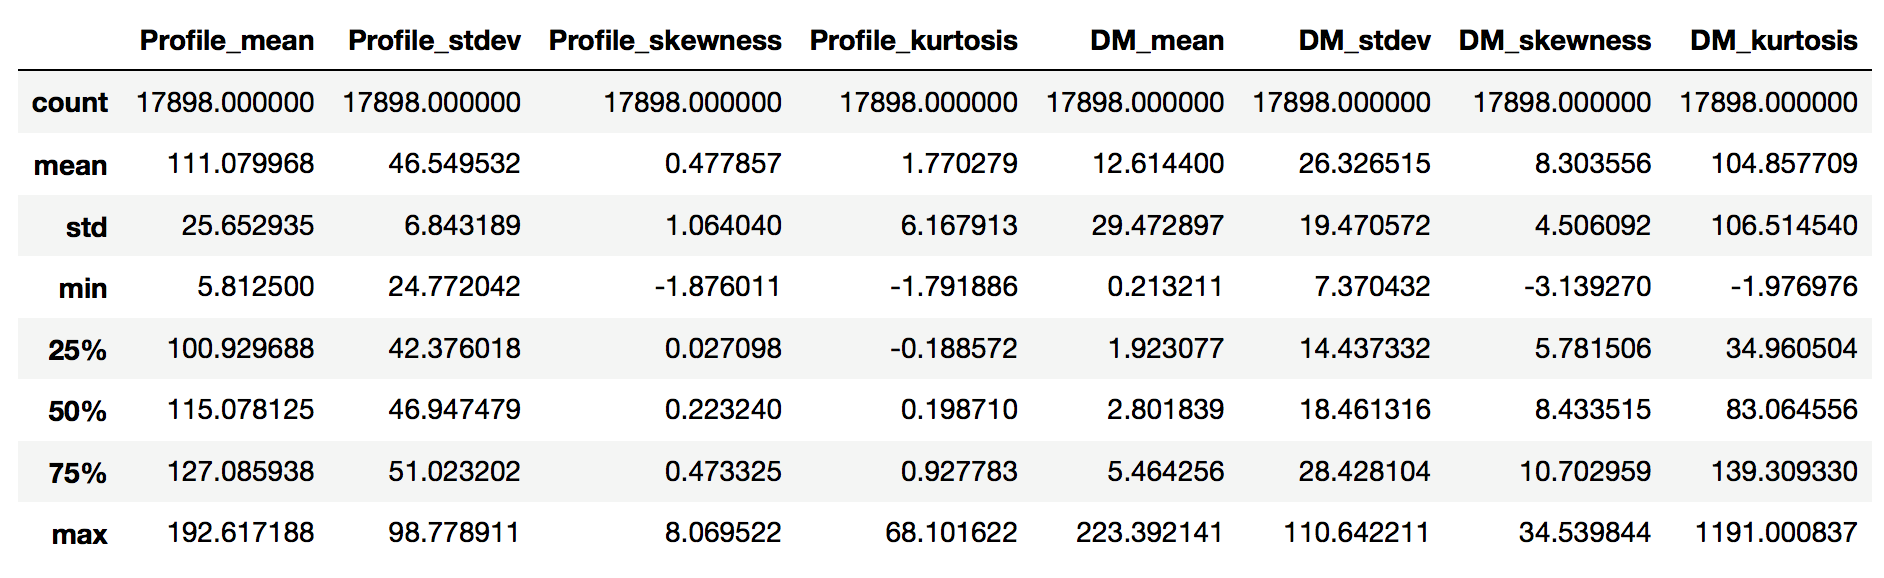
\includegraphics[scale=0.24]{img/distTable.png}
    \caption{Estatísticas descritivas sumárias, relativas às 8 variáveis de \textit{input}.}
    \label{fig:descricao_do_dataset}
    \end{figure}


\subsection{Pré-processamento dos dados.}
\label{sec:preprocessamento}
	Nesta secção, é descrito qual o pré-processamento aplicado ao conjunto de dados, explicando também as vantagens que daí advêm.

	Relativamente à etapa de pré-processamento dos dados, temos duas considerações importantes: por um lado, todas as colunas de \textit{input} contêm valores de vírgula flutuante, de distribuição contínua; por outro lado, a coluna de \textit{output}, corresponde a uma de duas classes (classe positiva ou negativa, caso seja ou não um pulsar).
    
    Assim, para facilitar a aprendizagem por parte do algoritmo e contribuir para convergir mais rapidamente, fazemos normalização dos dados de input (\textit{feature scaling}), para uma escala no alcance [-1,1]. Por sua vez, relativamente à classe de \textit{output}, extraímos os dados para uma matriz unidimensional em que cada elemento tem um valor binário: 1 caso seja referente a um pulsar, e 0 em caso contrário.

\subsection{Modelo de aprendizagem a aplicar: redes neuronais.}
\label{sec:redes_neuronais}
	Neste trabalho iremos usar uma rede neuronal artificial, \textit{Multilayer Perceptron} (MLP), que segue uma técnica de \textit{aprendizagem supervisionada} denominada \textit{backpropagation}. Assim, torna-se importante esclarecer cada um destes conceitos.

    Algoritmos que seguem o modelo da aprendizagem supervisionada são algoritmos nos quais os possíveis \textit{outputs} do algoritmo já são conhecidos e nos quais os dados usados para treinar o algoritmo já se encontram mapeados à resposta correta. Pode-se verificar que este modelo é aplicável ao problema dos pulsares na medida em que a totalidade das entradas na base de dados se encontram mapeados a um resultado, como na Secção~\ref{sec:dataset}.
    
    Por sua vez, \textit{backpropagation} é um método usado para o cálculo do gradiente de funções que regem as redes neuronais, sendo frequentemente usado no algoritmo de \textit{gradient descent}. Este é um algoritmo iterativo de otimização de primeira ordem, que permite encontrar o mínimo local de uma função.
    
	Dada uma rede neuronal artificial e uma função de erro (ou função de perda), o algoritmo de \textit{backpropagation}, também conhecido por algoritmo da propagação de erros para trás (\textit{backward propagation of errors}), calcula o gradiente da função de erro considerando sempre o peso das arestas na rede neuronal. Este cálculo é propagado para trás na rede neuronal, com o gradiente da última camada de pesos a ser calculado primeiro e o gradiente da primeira camada de pesos em último lugar (daí o seu nome \textit{backpropagation}). Este fluxo invertido da informação de erro permite uma computação eficiente do gradiente em cada camada, ao invés da abordagem ingénua de calcular o gradiente de cada camada separadamente.
    
    O algoritmo desenvolve-se em duas fases. Numa primeira fase, propaga-se através da rede de forma a chegar aos valores de \textit{output}. De seguida, calcula o custo da propagação para cada output, sendo que esta estará intrinsecamente relacionada com a função de erro usada no algoritmo do gradiente descendente. Por fim, propaga-se em sentido contrário de forma a gerar um valor de erro para cada um dos neurónios. Na segunda fase, os pesos das arestas são constantemente atualizados conforme o resultado desempenhado por cada um dos candidatos. Na atualização das arestas é usado uma percentagem previamente definida como fator de atualização dos pesos. Quanto mais elevado for este fator, mais rápido será o treino da rede neural. Por outro lado, quanto mais baixo for este fator, mais preciso será o treino.
    
% Durante o desenvolvimento deste projeto, foram implementados dois modelos de aprendizagem: um primeiro em que as três camadas eram do tipo \textit{Convolutional}, \textit{Dense} e \textit{Dense}
    
\subsection{Arquitetura das redes neuronais.}
\label{sec:arquitetura}
	As redes neuronais, surgiram com base na perceção biológica das interligações presentes no cérebro humano. Assim, tal como o cérebro humano é constituído por neurónios, os quais recebem impulsos nervosos como entrada e saída de dados, também as redes neuronais são constituídas por camadas de neurónios, ativados com estímulos específicos. Um neurónio tem a capacidade de estimular os seus neurónios vizinhos, quando este é propriamente estimulado (função de ativação). Posto isto, podemos definir matematicamente um neurónio como sendo:
    \begin{figure}[H]
    \centering
    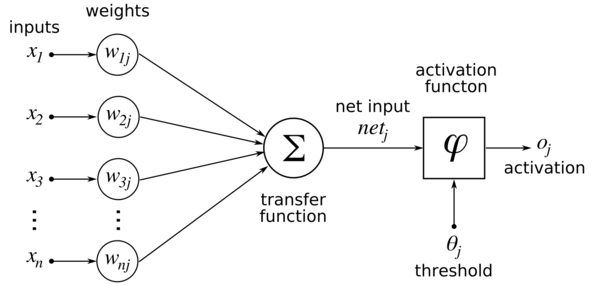
\includegraphics[scale=.5]{img/neural.png}
    \caption{Modelo natemático de um neurónio.}
    
    \LARGE{\[ y = f_\textit{ativação} (\sum_{i} w_ix_i - \theta ) \]}
    \caption{Representação matemática da saída de um neurónio.}
    \end{figure}
    
    Como o nome indica, é uma rede, por isso a sua consistência detêm vários neurónios conectados na forma de um grafo acíclico. As redes neuronais mais comuns, \textit{feedforward}, são redes em que o \textit{output} dos neurónios de uma camada é o \textit{input} dos neurónios da camada seguinte.

Desta forma é possível separar a rede em diferentes camadas:
	\begin{enumerate}
		\item Uma \textbf{\textit{Input Layer}}, primeira camada na rede neuronal, responsável por receber os dados, determinar o tamanho do \textit{dataset} e apresentar os padrões de reconhecimento. São apenas constituídas por neurónios de \textit{input}.
		\item Uma ou mais \textbf{\textit{Hidden Layer}}, é nesta(s) camada(s) que é feita maior parte da aprendizagem dos pesos do modelo. Camadas seguidas deverão corresponder a \textit{features} cada vez mais abstratas, permitindo alcançar um modelo generalizável e de bom desempenho.
        \item Uma \textbf{\textit{Output Layer}}, última camada da rede, responsável por apresentar os dados, esta camada é constituída com um número de neurónios geralmente igual ao número de classes de \textit{output} (ou apenas 1 se se tratar de classificação binária). É uma camada que não dispõe de função de ativação, e os cujos são exclusivamente neurónios de \textit{output}.
	\end{enumerate}
    
    \begin{figure}[H]
    \centering
    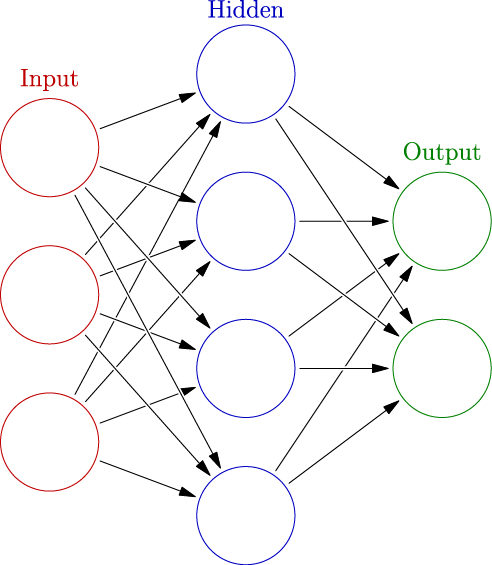
\includegraphics[scale=.7]{img/neural_network.png}
    \caption{Representação Abstrata da Rede Neural}
    \end{figure}
    
\subsection{Configuração da rede neuronal.}
\label{sec:configuracao_rede}
    Partindo agora para o nosso caso em concreto, é sempre muito complicado prever a configuração/arquitetura da rede ideal para um dado problema, isto é, qual o número ideal de \textit{hidden layers}, qual o número de neurónios das camadas, qual o tipo de funções de ativação usadas, entre outras variações. Por isso é algo que requer alguns testes com diferentes composições para se obter os melhores resultados, coadjuvados por métodos de \textit{Grid Search}, testando um conjunto de combinações promissoras e melhorando iterativamente.
    
    Neste sentido, foram desenvolvidos testes ao número de \textit{hidden layers}, variando entre 1 a 2 o número destas \textit{layers}, e variando também o número de neurónios em cada uma entre 8, 12, 16, ou 32. Como função de ativação, foi usada a função ``relu'' para as camadas intermédias (\textit{hidden}).
    A camada de \textit{input} terá obrigatoriamente 8 entradas (uma por variável), e a camada de \textit{output} tem apenas 1 neurónio, ativado pela função ``sigmoid'', de modo a balisar o \textit{output} entre 0 e 1 (indicativo do grau de certeza de o candidato se tratar ou não de um pulsar).
    Os resultados destas configurações são apresentados na Secção~\ref{sec:experiencias}.

\subsection{Forma de Avaliação}
\label{sec:avaliacao}
Para nos assegurarmos que o modelo cumpre os requisitos, todos os dados reportados são resultantes de \textit{k-fold cross-validation} (validação cruzada em \textit{k} partes). Assim, numa fase inicial usamos \textit{cross-validation} com $k=3$ (para um treino mais rápido dos modelos, e assim uma pesquisa mais rápida sobre os possíveis hiperparâmetros), e, após terem sido identificados alguns modelos promissores, prosseguimos com $k=5$.

Adicionalmente, e tendo em conta a tarefa em questão, será muito útil ter em atenção o \textit{recall} da classe positiva, pois queremos maximizar a identificação de pulsares. Neste sentido, as métricas usadas para avaliação dos modelos serão numa primeira fase a exatidão global do modelo (\textit{accuracy}), e numa segunda fase uma avaliação mais detalhada com o \textit{recall} da classe positiva, e o \textit{F1 score}. O \textit{F1 score} consiste numa média harmónica da precisão e do \textit{recall} para cada uma das classes em causa.


\section{Desenvolvimento}
\label{sec:desenvolvimento}
Nesta secção, será analisado o desenvolvimento do trabalho em si, nomeadamente quais as ferramentas e linguagens de programação utilizadas, qual a estrutura da aplicação concebida e os detalhes da sua implementação.

\subsection{Ferramentas utilizadas}

Para o desenvolvimento da aplicação foi usada a linguagem de programação \textit{Python3}.

Foram usadas várias bibliotecas da linguagem referida, sendo de importante menção as seguintes: \textit{keras}, para modelação rápida de alto nível da rede neuronal; \textit{Tensorflow}, para modelação de baixo nível da rede neuronal, proporcionando maior liberdade em detrimento do tempo de desenvolvimento; \textit{scikit-learn}, para análise dos modelos gerados, realização de validação cruzada e cálculo de métricas globais como \textit{F1-score}; \textit{imblearn}, útil no manuseamento de conjuntos de dados desequilibrados, possibilitando fácil reamostragem dos dados usados na aplicação, nomeadamente \textit{undersampling}; \textit{numpy}, para execução de operações sobre matrizes com elevada \textit{performance}; \textit{matplotlib} para criação de diversos gráficos (\textit{e.g.} Figura~\ref{fig:distribuicoes}); finalizando, \textit{tensorboard}, para visualização de métricas e do seu progresso no decorrer do treino, bem como visualização das ativações de neurónios da rede neuronal.

Outras bibliotecas usadas, mas de menor relevância, são ainda: \textit{absl-py}, \textit{astor}, \textit{bleach}, \textit{gast}, \textit{grpcio}, \textit{h5py}, \textit{html5lib}, \textit{pandas}, \textit{protobuf}, \textit{python-dateutil}, \textit{pytz}, \textit{PyYAML}, \textit{scipy}, \textit{six}, \textit{termcolor} e \textit{Werkzeug}.

A aplicação foi ainda desenvolvida e testada em três sistemas operativos, nomeadamente, Linux, MacOS e Windows. 

\subsection{Estrutura da aplicação}

É possível dividir o trabalho em cinco fases distintas:
\begin{enumerate}
	\item Carregamento dos dados e repartição dos mesmos em dados de treino e de teste, de forma a melhor controlar o fenómeno de \textit{overfitting}.
	\item Aplicação opcional de \textit{undersampling}.
	\item Criação do modelo da rede neuronal.
	\item Treino da rede neuronal.
	\item Avaliação da rede neuronal.
    \item Geração de gráficos referentes ao treino e teste da rede neuronal.
\end{enumerate}

Através da análise do ficheiro \textit{main.py}, é possível distinguir as respetivas chamadas as quatro fases referidas. 

Assim, para a primeira fase referida - carregamento dos dados e repartição dos mesmos -, a respetiva secção de código é:

\begin{lstlisting}[language=python]
pulsars = load_pulsar_csv()
train_set, test_set = train_test_split(pulsars, 0.2)

X_train, Y_train = train_set[:, :-1], train_set[:, -1]
X_test, Y_test = test_set[:, :-1], test_set[:, -1]
\end{lstlisting}

Neste excerto de código, começamos por guardar na variável \textit{pulsar} os dados que nos são fornecidos. de seguida dividimos esses dados, em dois conjuntos, os dados usados para testar a rede neuronal e os dados usados para avaliação da rede neuronal. Nas duas linhas seguintes, definimos o \textit{input} e o \textit{output} para cada um dos conjuntos previamente criados.

Para a segunda fase referida - Aplicação de \textit{undersampling} -, a respetiva secção de código é:
\begin{lstlisting}[language=python]
from imblearn.under_sampling import RandomUnderSampler
rus = RandomUnderSampler(return_indices=True)
X_resampled, Y_resampled, idx_resampled = rus.fit_sample(pulsars[:,:-1], pulsars[:,-1])
print("Original data size: %d. Undersampled data size: %d" % (len(pulsars), len(X_resampled)))

X_train, Y_train = X_resampled, Y_resampled
\end{lstlisting}
Antes de procedermos à explicação do excerto de código apresentado, consideramos necessário deixar transparente o que é \textit{undersampling}. Por \textit{undersampling} entende-se a eliminação aleatória de dados da classe maioritária, de forma a reduzir o impacto desta sobre o conjunto de dados.

Neste excerto de código, são criadas duas variáveis de \textit{input} e \textit{output} resultantes da aplicação de \textit{undersampling} ao conjunto de dados, sendo estas posteriormente usadas como \textit{input} e \textit{output} do conjunto de treino.

Para a terceira fase referida - criação do modelo da rede neuronal -, a respetiva secção de código é:
\begin{lstlisting}[language=python]
model = create_model(np.size(X_train, axis=1))
\end{lstlisting}
A função \textit{create\_model} encontra-se definida no ficheiro \textit{modes.py}, sendo a sua definição:
\begin{lstlisting}[language=python]
def create_model(input_dim):
    input = Input(shape=(input_dim,))
    x = Dense(32)(input)
    x = LeakyReLU(alpha=0.3)(x)
    x = Dense(16)(x)
    x = Activation('relu')(x)
    output = Dense(1, activation='sigmoid')(x)

    model = Model(inputs=input, outputs=output)
    model.compile(optimizer='adam', loss='binary_crossentropy', metrics=['accuracy'])
    return model
\end{lstlisting}
Neste excerto de código, é definido o modelo a ser utilizado pela rede neuronal. Este é constituído por duas camadas, tendo a primeira um total de trinta e dois neurónios e a segunda dezasseis neurónios. Na secção~\ref{sec:experiencias} será feita uma análise minuciosa sobre o modelo usado.

Para a quarta fase referida - treino da rede neuronal -, a respetiva secção de código é:
\begin{lstlisting}[language=python]
## Optionally: Balance Class Weights
from sklearn.utils import class_weight
class_weight = class_weight.compute_class_weight('balanced',
                                                 np.unique(Y_train),
                                                 Y_train)
print("Class weight: ", class_weight)
#

# Train Model
model.fit(X_train, Y_train, epochs=100, batch_size=16,
        validation_data=(X_test, Y_test),
        callbacks=callbacks,
        class_weight={0: class_weight[0], 1: class_weight[1]}
        )
\end{lstlisting}
Neste excerto de código, o modelo criado é treinado usando o conjuntos de dados de treino previamente computados. Estes encontram-se guardados nas variáveis \textit{X\_train} e \textit{Y\_train}. De notar que é efetuado um estudo em relação ao peso das classes, sendo este detalhadamente explicado na secção~\ref{sec:experiencias}.

Para a quinta fase referida - avaliação da rede neuronal -, a respetiva secção de código é:
\begin{lstlisting}[language=python]
scores = model.evaluate(X_test, Y_test)
print("Overall Accuracy: %.2f\n" % (scores[1] * 100))
print(evaluate_classwise(model, X_test, Y_test))
\end{lstlisting}
Neste excerto de código, é feita a avaliação do modelo usando o conjunto de dados previamente guardados nas variáveis \textit{X\_test} e \textit{Y\_test}. Posteriormente, é também avaliado o desempenho do modelo em cada classe (precisão, \textit{recall}, \textit{F1-score}).

\subsection{Detalhes de Implementação}
Para além do uso normal da plataforma \textit{TensorBoard}, foi extendida com ajuda a software de código livre de modo a facilitar a criação de gráficos e outras visualizações. Esta extensão foi feita por herança da classe \textit{keras.callbacks.TensorBoard}, disponível no ficheiro \textit{PRTensorBoard.py}. Após esta definição, apenas é necessário passar uma instância da classe aos callbacks de treino do modelo.

\begin{lstlisting}[language=python]
callbacks = [
        PRTensorBoard(log_dir=('../Graph/' + MODEL_NAME), write_images=True, histogram_freq=5),
        EarlyStopping(monitor='val_acc', patience=20)
        ]
\end{lstlisting}

\begin{figure}[h!]
\centering
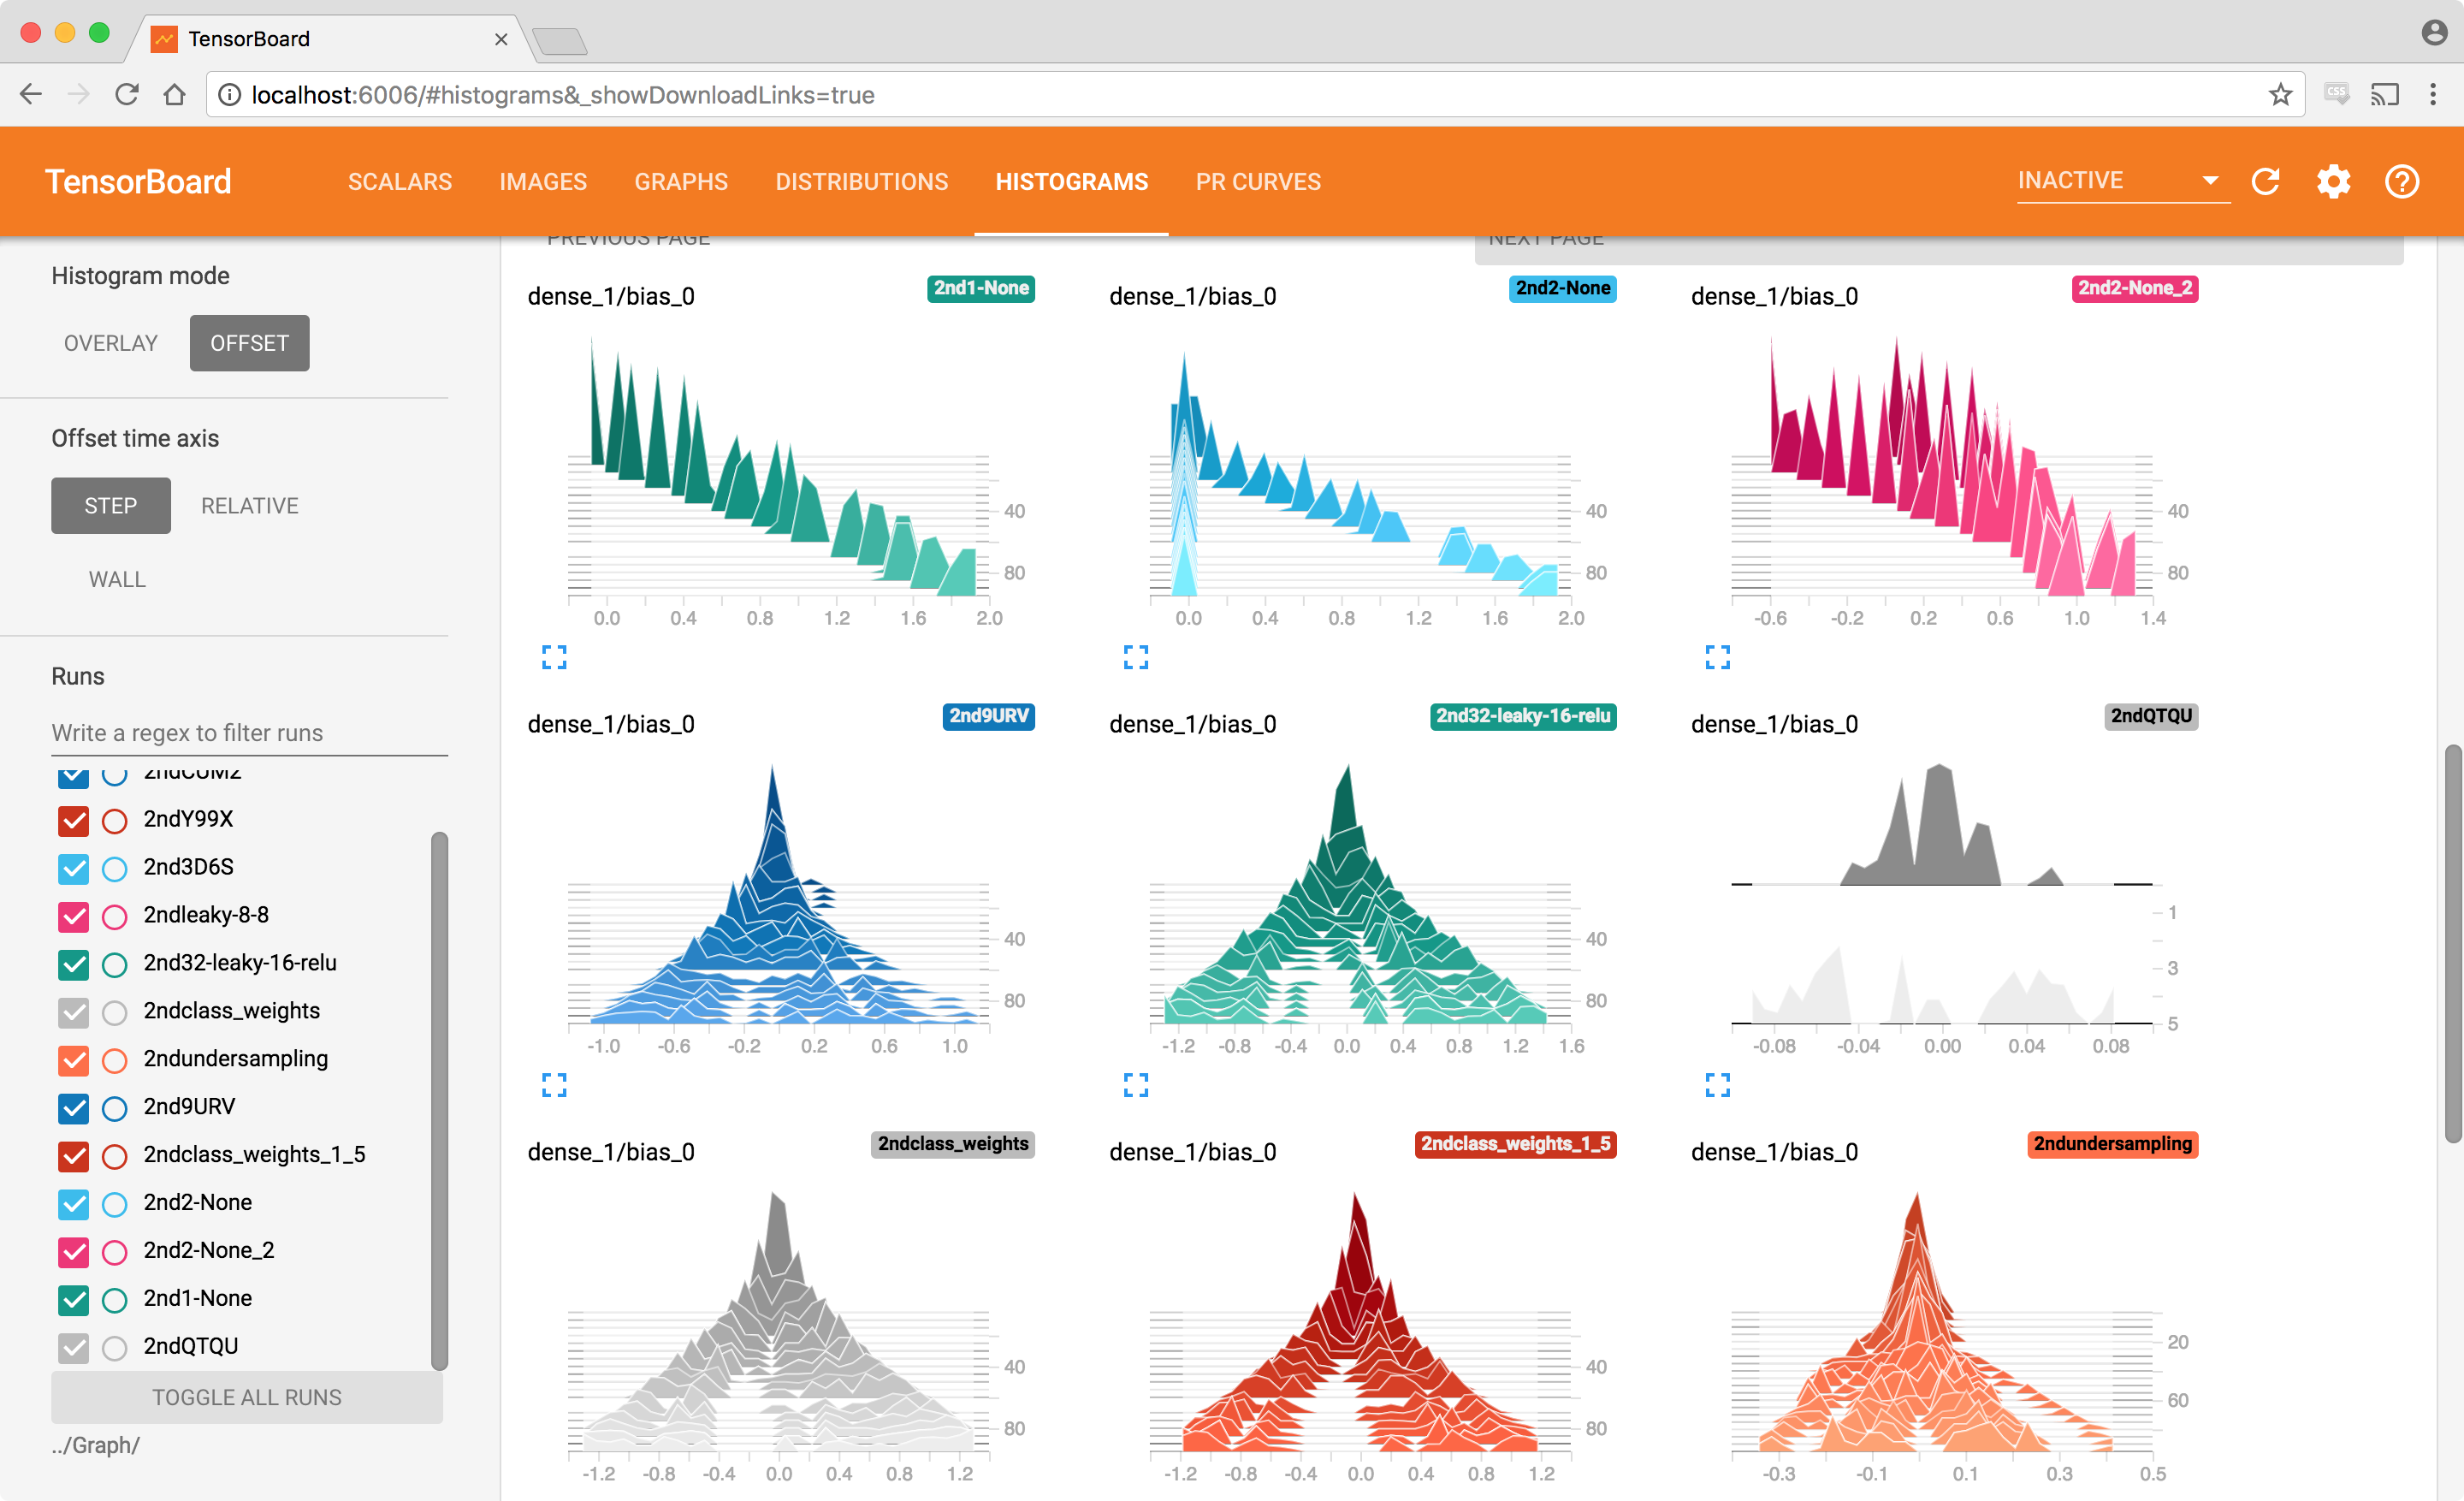
\includegraphics[scale=0.25]{img/tensorboard.png}
\caption{Interface do TensorBoard.}
\label{fig:tensorboard}
\end{figure}


\section{Experiências}
\label{sec:experiencias}
Esta secção expõe detalhadamente todas as experiências feitas para melhor solucionar o problema de classificação de pulsares. Para isso, como visto nas secções anteriores, iremos utilizar redes neuronais artificiais \textit{feedforward}. Neste sentido, as experiências incidem sobre o tamanho das \textit{hidden-layers}, as suas funções de ativação, a função de treino utilizada, e, por último, técnicas para equilibrar as duas classes de um \textit{dataset} desequilibrado. Para além disso, todas as redes geradas têm algumas características em comum:
\begin{itemize}
\item Uma camada de entrada, com 8 neurónios (1 por cada \textit{feature} de que dispomos);
\item Uma camada de saída, com 1 neurónio, ativada pela função \textit{sigmoid}, de modo a que o output da rede seja a probabilidade de a instância em causa ser um pulsar;
\item Uma ou duas camadas escondidas, de tamanho variável;
\item A função de perda será \textit{binary crossentropy};
\item A \textit{seed} de aleatoriedade foi fixada no valor 42, para ser possível reproduzir facilmente os resultados;
\end{itemize}


\subsection{Tamanho das \textit{Hidden-Layers}}
\label{sec:tamanho_das_layers}
Esta experiência teve como objetivo determinar qual o melhor número de neurónios das camadas escondidas da rede. Neste sentido foi feita uma pesquisa exaustiva (\textit{grid search}) sobre um conjunto de tamanhos que achamos promissores. Os resultados, obtidos ao fim de 100 \textit{epochs} e validados por \textit{3-fold cross-validation}, estão apresentados na Tabela~\ref{tab:grid_search_hidden_layers}.

\begin{table}[h!]
\centering
  \begin{tabular}{lll}
  \hline
  First Hidden Layer & Second Hidden Layer & Accuracy \\ \hline
  32                 & 16                 & 97.93    \\
  32                 & 12                 & 97.57    \\
  32                 & 4                  & 97.58    \\
  32                 & 2                  & 97.50    \\
  32                 & -                  & 97.49    \\
  16                 & 16                 & 97.87    \\
  16                 & 12                 & 97.52    \\
  16                 & 4                  & 97.46    \\
  16                 & 2                  & 97.17    \\
  16                 & -                  & 97.31    \\
  8                 & 16                  & 97.69    \\
  8                 & 12                  & 97.52    \\
  8                 & 4                   & 97.16    \\
  8                 & 2                   & 97.21    \\
  8                 & -                   & 97.11    \\
  4                 & 16                  & 97.65    \\
  4                 & 12                  & 97.54    \\
  4                 & 4                   & 97.36    \\
  4                 & 2                   & 97.12    \\
  4                 & -                   & 96.97    \\
  2                 & 16                  & 96.99    \\
  2                 & 12                  & 97.02    \\
  2                 & 4                   & 96.94    \\
  2                 & 2                   & 96.76    \\
  2                 & -                   & 96.50    \\ \hline \\
  \end{tabular}
  \caption{Resultados obtidos com diferentes configurações da rede neuronal, por ordem decrescente da primeira coluna, e de seguida por ordem decrescente da segunda coluna.}
  \label{tab:grid_search_hidden_layers}
\end{table}

Como podemos ver, atingimos resultados muito promissores, sendo que o melhor modelo obteve exatidão de 97.93\%, e tem duas \textit{hidden layers}, a primeira com 32 neurónios e a segunda com 16 neurónios. Como indicado no início desta secção, esta experiência é facilmente reproduzível, pois a \textit{seed} de aleatoriedade foi fixada no valor 42.

Adicionalmente, é importante notar que a diferença entre os desempenhos dos diferentes modelos é diminuta, tendo a esmagadora maioria das configurações de rede resultado em valores de exatidão entre 97\% e 98\%. O desempenho de alguns modelos ao longo dos \textit{epochs} de treino está disponível na figura~\ref{fig:acc_grid_search_layers_size}, mostrando apenas as arquiteturas do tipo x-16 para não poluir o gráfico, mantendo os dados interpretáveis. A perda dos mesmos modelos ao longo dos \textit{epochs} de treino está disponível na figura~\ref{fig:loss_grid_search_layers_size}.

\begin{figure}[h!]
\centering
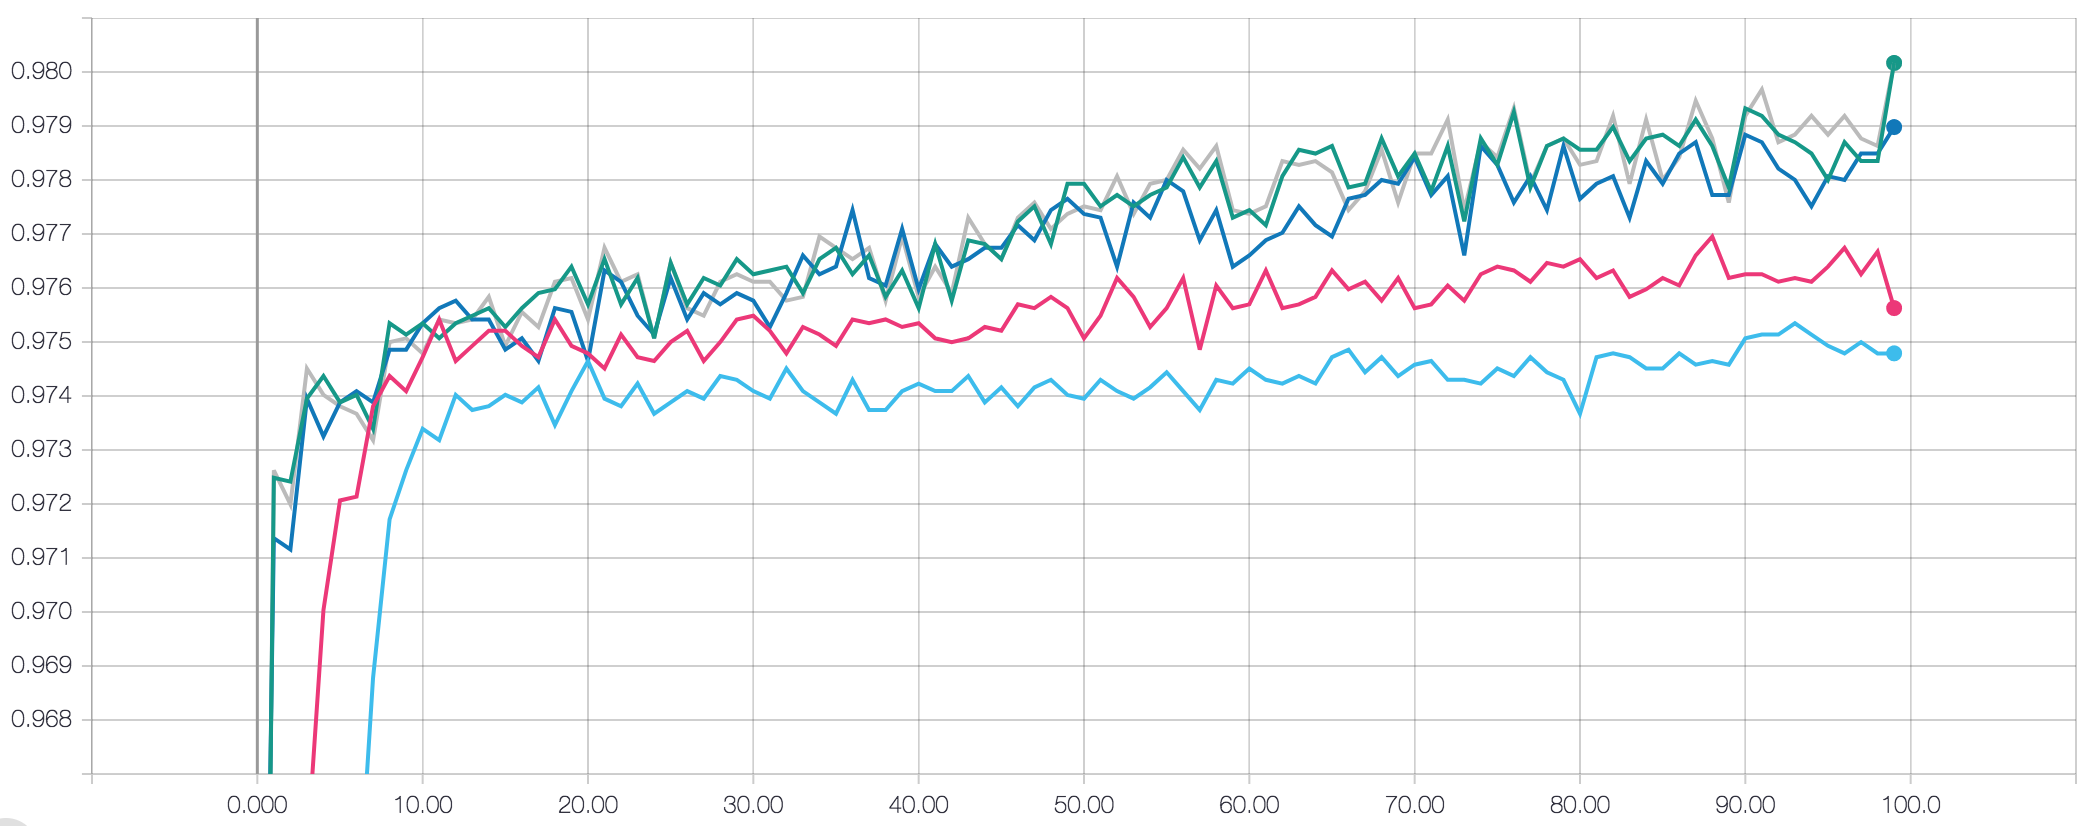
\includegraphics[scale=0.35]{img/acc_grid_search_selected_models.png}
\caption{Exatidão dos modelos em função do número de \textit{epochs} de treino, medida num dataset reservado para validação. Legenda: a cinzento a arquitetura 32-16; a verde a arquitetura 16-16; a azul escuro a arquitetura 8-16; a magenta a arquitetura 4-16; e a azul claro a arquitetura 2-16.}
\label{fig:acc_grid_search_layers_size}
\end{figure}

\begin{figure}[h!]
\centering
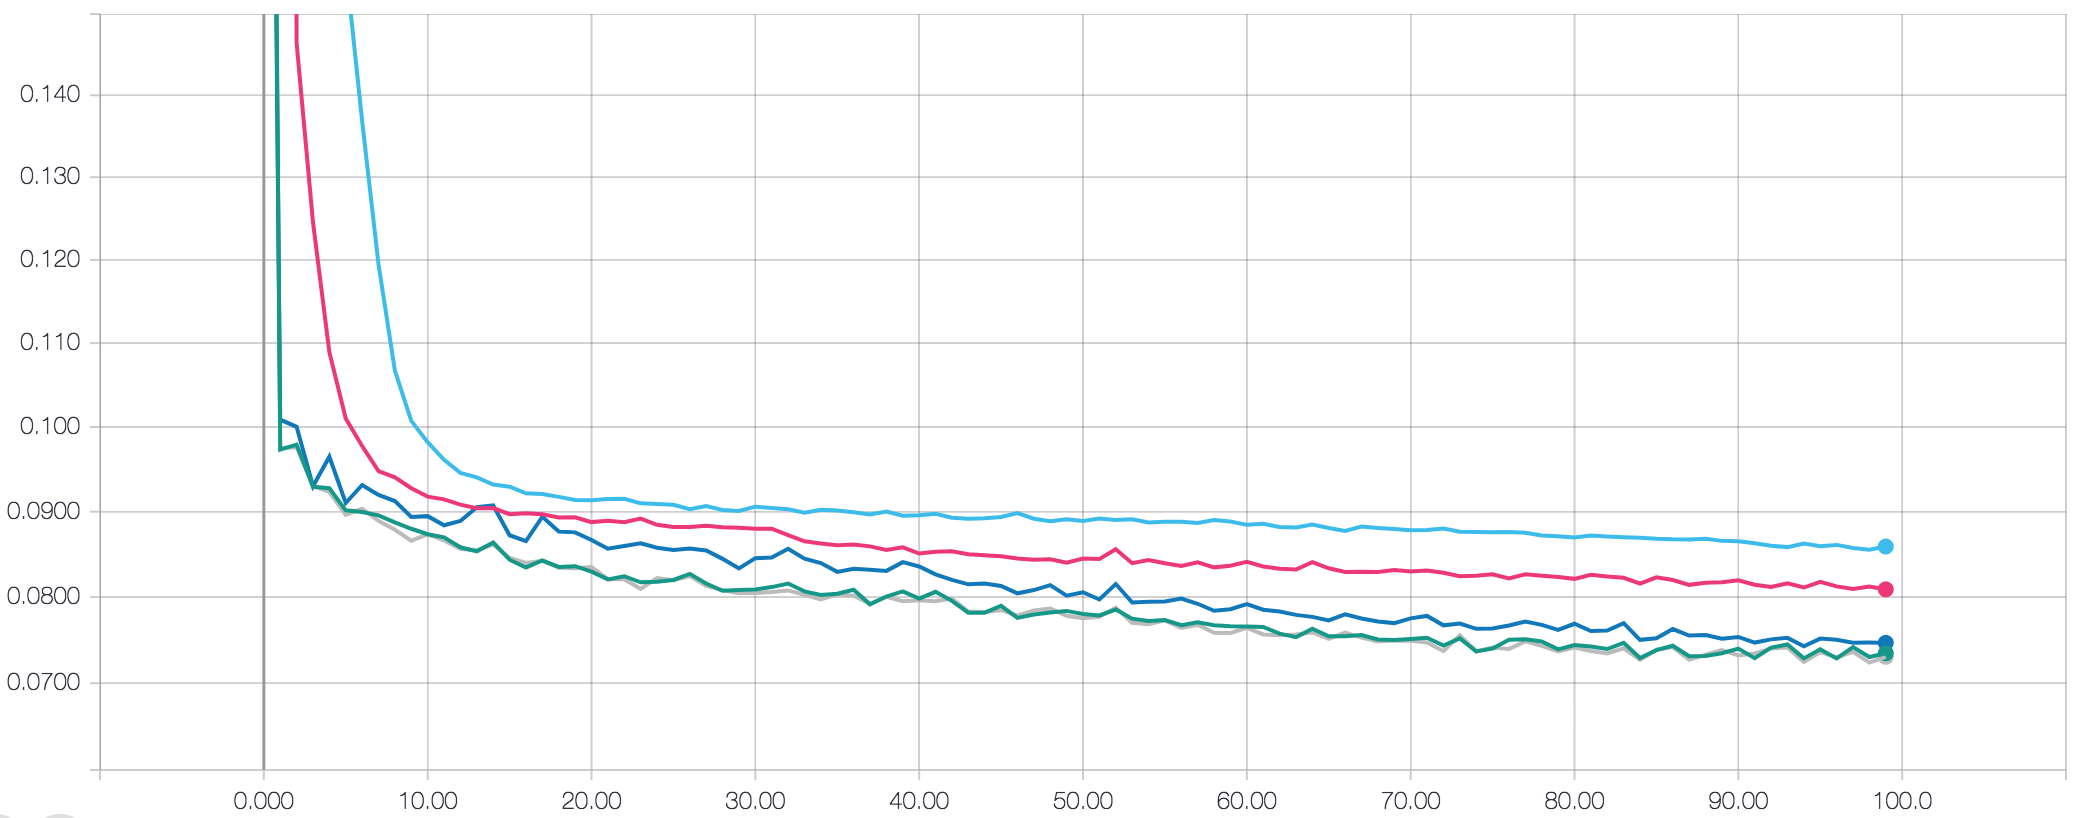
\includegraphics[scale=0.35]{img/loss_grid_search_selected_models.png}
\caption{Perda dos modelos em função do número de \textit{epochs} de treino, medida num dataset reservado para validação. Legenda: a cinzento a arquitetura 32-16; a verde a arquitetura 16-16; a azul escuro a arquitetura 8-16; a magenta a arquitetura 4-16; e a azul claro a arquitetura 2-16.}
\label{fig:loss_grid_search_layers_size}
\end{figure}

É também interessante notar que uma rede muito simples, com apenas uma \textit{hidden layer} com dois neurónios, conseguiu um valor de exatidão de 96.50\%, apenas 1.43\% menos do que o melhor modelo.
Achamos que isto se deve ao diminuto tamanho do \textit{dataset} que usamos, não sendo suficiente para treinar modelos mais complexos, e portanto não aproveitando todo o potencial de que um modelo com duas \textit{hidden layers} dispõe. Para além disso, também estará relacionado com a distribuição das classes no \textit{dataset} (a classe negativa representa cerca de 91\% dos dados), o que faz com que facilmente se atinjam os 91\% de exatidão. No entanto, é importante notar que os modelos mais complexos não sofreram overfitting, alcançando os melhores valores de desempenho, e sendo estáveis ao longo da validação cruzada (\textit{cross validation}).


\subsection{Algoritmos de Otimização de \textit{Gradient Descent}}
\label{sec:optimizers}
Esta experiência teve como objetivo determinar qual o melhor algoritmo de otimização de \textit{gradient descent} a usar, de entre elas: \textit{RMSprop}, \textit{Adam}, \textit{AdaMax}, \textit{Nadam}, \textit{Adadelta}, ou simplesmente \textit{Stochastic Gradient Descent}. Foram usados apenas algumas configurações de rede selecionadas da experiência anterior, de modo a controlar o tempo de computação (acabando por demorar cerca de 3 horas). Os resultados, obtidos ao fim de 100 \textit{epochs} e validados por \textit{3-fold cross-validation}, estão apresentados na Tabela~\ref{tab:grid_search_optimizers}.

\begin{table}[h!]
\centering
  \begin{tabular}{llll}
  \hline
  Optimizer & First Hidden Layer & Second Hidden Layer & Accuracy \\ \hline
  SGD		& 32                 & 16                 & 94.23    \\
  RMSprop	& 32                 & 16                 & 96.63    \\
  Adadelta	& 32                 & 16                 & 97.66    \\
  Adam		& 32                 & 16                 & 90.36    \\
  AdaMax	& 32                 & 16                 & 97.68    \\
  Nadam		& 32                 & 16                 & 90.52    \\ \hline
  SGD		& 32                 & 8                 & 97.43    \\
  RMSprop	& 32                 & 8                 & 97.76    \\
  Adadelta	& 32                 & 8                 & 97.72    \\
  Adam		& 32                 & 8                 & 93.21    \\
  AdaMax	& 32                 & 8                 & 97.75    \\
  Nadam		& 32                 & 8                 & 96.75    \\ \hline
  SGD		& 32                 & 4                 & 95.74    \\
  RMSprop	& 32                 & 4                 & 97.83    \\
  Adadelta	& 32                 & 4                 & 96.35    \\
  Adam		& 32                 & 4                 & 96.24    \\
  AdaMax	& 32                 & 4                 & 97.77    \\
  Nadam		& 32                 & 4                 & 97.94    \\ \hline \\
\end{tabular}
  \caption{Valores de exatidão de modelos treinados com diferentes funções de otimização de treino, separados por diferentes configurações da rede neuronal.}
  \label{tab:grid_search_optimizers}
\end{table}


Os resultados obtidos são algo surpreendentes, mostrando a instabilidade de treino de configurações de rede maiores: a configuração 32-16 obteve valores inconsistentes, enquanto a configuração 32-4 obteve consistentemente bons resultados. Esta inconsistência deve-se possivelmente à maior dificuldade por parte de maiores redes neuronais de escaparem a estados de equilíbrio locais.

O melhor resultado  desta pesquisa exaustiva de hiperparâmetros foi obtido pelo conjunto (Nadam, 32, 4), ou seja, o otimizador \textit{Nadam}, com uma rede com 32 neurónios na primeira camada escondida, e 4 neurónios na segunda camada escondida. Este valor é consideravelmente melhor que o previamente obtido para esta configuração ($97.94 > 97.58$). Este conjunto foi ainda testado mais exaustivamente, com os dados de precision, recall, e \textit{f1} de cada classe disponíveis na tabela~\ref{tab:nadam_32_4}.

\begin{table}[h!]
\centering
  \begin{tabular}{llll}
  \hline
   				  & \textit{Precision} & \textit{Recall} & \textit{F1} \\ \hline
  Classe Negativa & 99			   & 99			 & 99   \\
  Classe Positiva & 92			   & 85			 & 88    \\ \hline \\
\end{tabular}
  \caption{Valores de \textit{precision}, \textit{recall} e \textit{F1-score} para a configuração de rede 32-4, treinada com o otimizador \textit{Nadam}.}
  \label{tab:nadam_32_4}
\end{table}



\subsection{Reamostragem dos Dados da Classe Maioritária}
\label{sec:undersampling_class_weights}
Uma das principais dificuldades deste problema é o facto de as frequências das duas classes serem extremamente desequilibradas (numa razão de 10 para 1). Para tentar colmatar esta dificuldade fizemos uso de duas técnicas: \textit{resampling} dos dados da classe maioritária (a classe negativa), de modo a igualar o número de instâncias da classe minoritária (a classe positiva); e a alteração da perda no treino do modelo consoante a classe, de modo a que cada instância da classe minoritária conte como 5 instâncias da classe maioritária. Os resultados do primeiro teste (de \textit{undersampling}) estão disponíveis na tabela~\ref{tab:undersampling}, e os resultados o segundo teste (de diferentes pesos para cada classe) estão disponíveis na tabela~\ref{tab:class_weights}.

\begin{table}[h!]
\centering
  \begin{tabular}{llll}
  \hline
   				  & \textit{Precision} & \textit{Recall} & \textit{F1} \\ \hline
  Classe Negativa & 89			   & 96			 & 92   \\
  Classe Positiva & 95			   & 87			 & 91    \\ \hline \\
\end{tabular}
  \caption{Valores obtidos num \textit{dataset} reamostrado, com número igual de instâncias de cada classe. Valores referentes à melhor configuração de rede da experiência anterior.}
  \label{tab:undersampling}
\end{table}

\begin{table}[h!]
\centering
  \begin{tabular}{llll}
  \hline
   				  & \textit{Precision} & \textit{Recall} & \textit{F1} \\ \hline
  Classe Negativa & 99			   & 98			 & 99   \\
  Classe Positiva & 84			   & 92			 & 88    \\ \hline \\
\end{tabular}
  \caption{Valores obtidos com treino com peso das classes modificado: erros na classe positiva valem 5 vezes mais que erros na classe negativa. Valores referentes à melhor configuração de rede da experiência anterior.}
  \label{tab:class_weights}
\end{table}

Os resultados obtidos estão em linha com o esperado, havendo um aumento generalizado do desempenho na classe positiva, acompanhado com uma diminuição do desempenho na classe negativa. É de particular importância o facto de a realização de \textit{undersampling} aumentar consideravelmente a precisão na classe positiva, de 92\% para 95\%, e diminui a precisão na classe negativa de 99\% para 89\%. É também interessante o facto de a modificação dos pesos das classes ter aumentado substancialmente o \textit{recall} da classe positiva, de 85\% para 92\%, mas piorado a precisão na mesma classe, de 92\% para 84\%, mantendo o score \textit{F1} nos 88\%.

\begin{figure}[h!]
\centering
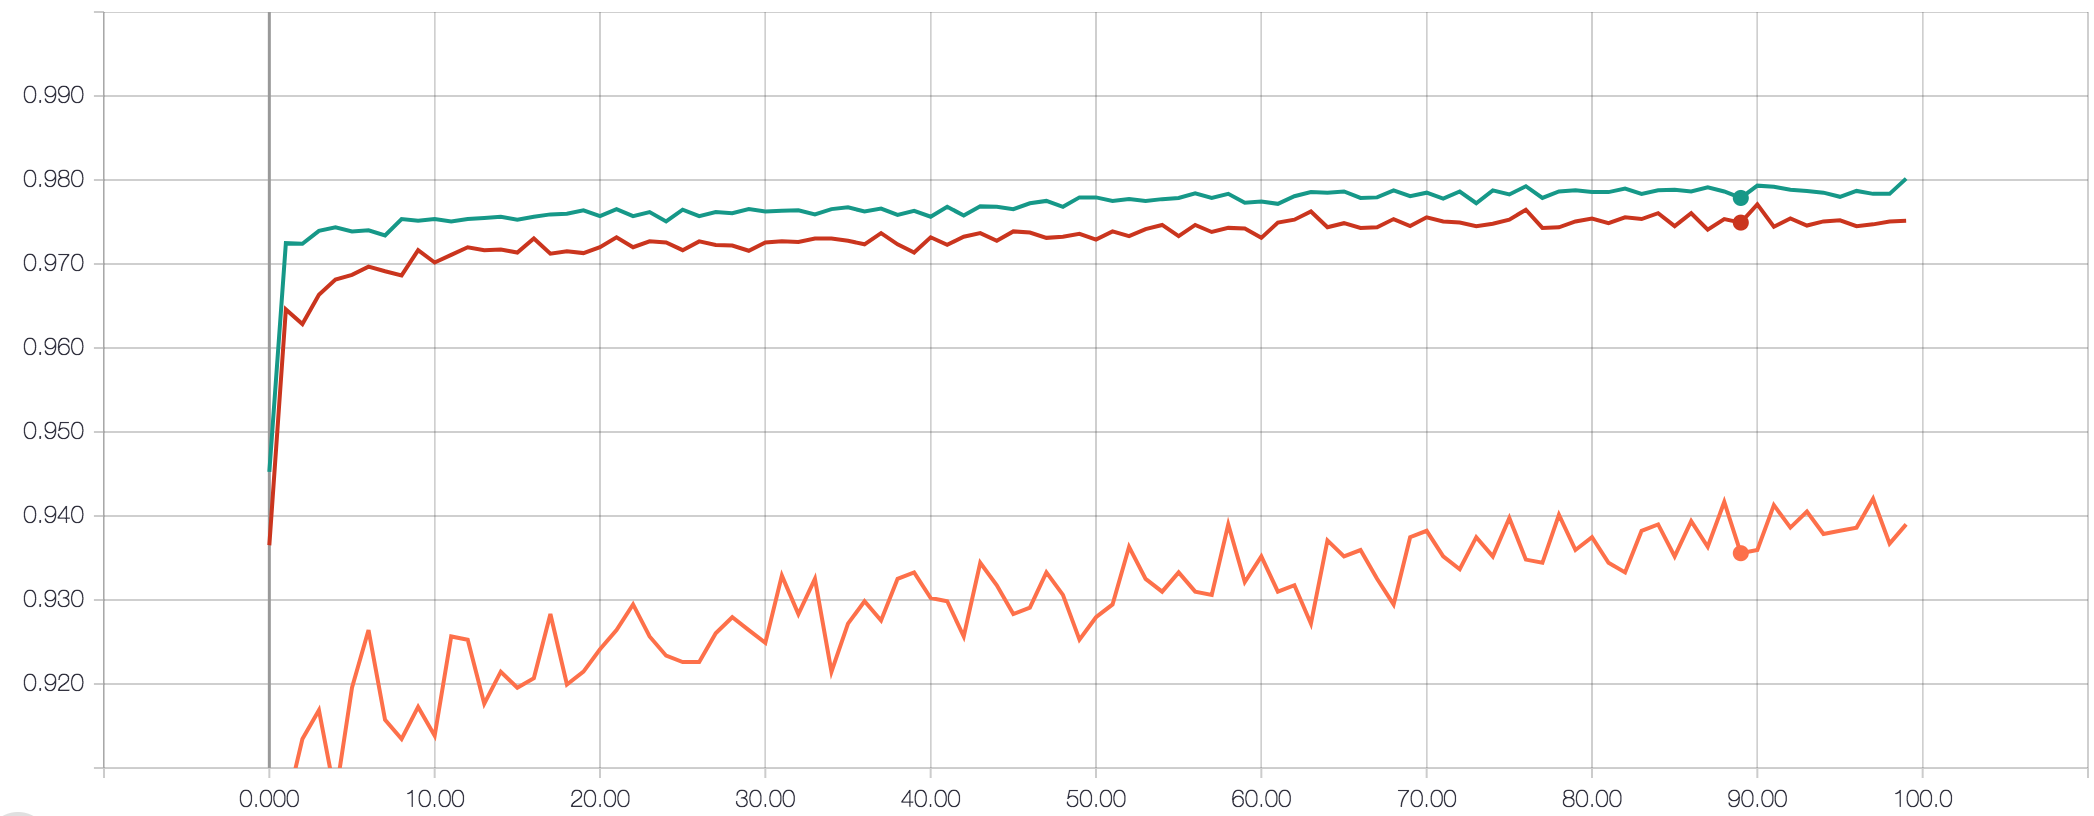
\includegraphics[scale=0.35]{img/acc_undersampling_class_weights.png}
\caption{Exatidão dos modelos em função do número de \textit{epochs} de treino, medida num dataset reservado para validação. Legenda: a verde o melhor modelo da experiência anterior (Secção~\ref{sec:optimizers}); a vermelho a experiência resultante da alteração dos pesos das classes (Tabela~\ref{tab:class_weights}); e a laranja a experiência resultante de \textit{undersampling} (Tabela~\ref{tab:undersampling}).}
\label{fig:acc_undersampling_class_weights}
\end{figure}

\begin{figure}[h!]
\centering
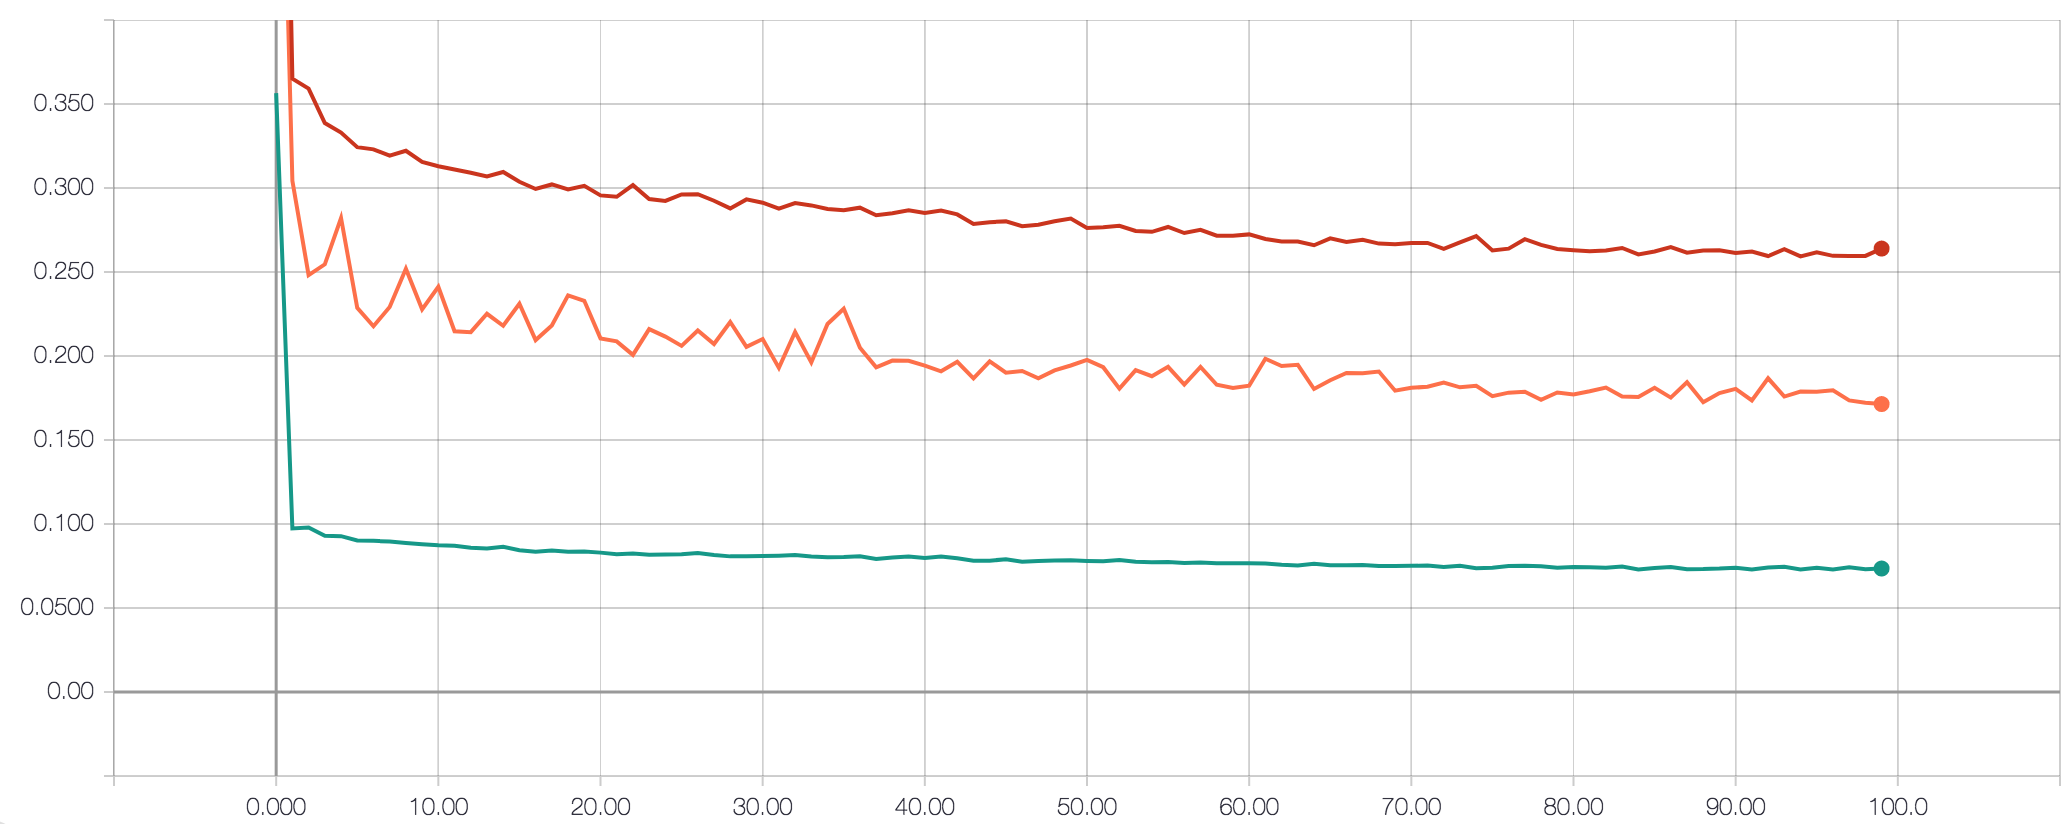
\includegraphics[scale=0.35]{img/loss_undersampling_class_weights.png}
\caption{Perda dos modelos em função do número de \textit{epochs} de treino, medida num dataset reservado para validação. Legenda: a verde o melhor modelo da experiência anterior (Secção~\ref{sec:optimizers}); a vermelho a experiência resultante da alteração dos pesos das classes (Tabela~\ref{tab:class_weights}); e a laranja a experiência resultante de \textit{undersampling} (Tabela~\ref{tab:undersampling}).}
\label{fig:loss_undersampling_class_weights}
\end{figure}

Adicionalmente, expomos os gráficos da precisão (Figura~\ref{fig:acc_undersampling_class_weights}) e da perda (Figura~\ref{fig:loss_undersampling_class_weights}) de ambos os modelos, bem como do melhor modelo da experiência anterior (Secção~\ref{sec:optimizers}) para comparação. É particularmente interessante o facto de o modelo que foi treinado com pesos de perda alterados nas diferentes classes ter melhor resultados que o modelo treinado nos dados \textit{undersampled}, no entanto ter também maior perda do que este, resultante de a perda na classe positiva contar 5 vezes mais para o primeiro modelo.


Achamos também interessante apresentar a curva de precisão da classe positiva em função do \textit{recall} da mesma classe, consoante o limiar de separação das duas classes é alterado, e que normalmente é 0.5 (Figura~\ref{fig:precision-recall_curve_normal_undersampled_class_weights}). É evidente a separação do modelo resultante de dados \textit{undersampled} dos restantes modelos, conseguindo uma melhor precisão a níveis de \textit{recall} próximos do máximo. Tendo isto em conta, podemos concluir que se o objetivo for a captação do maior número possível de instâncias de Pulsar, este será o modelo mais indicado, obrigando no entanto a uma posterior triagem de falsos positivos.

\begin{figure}[h!]
\centering
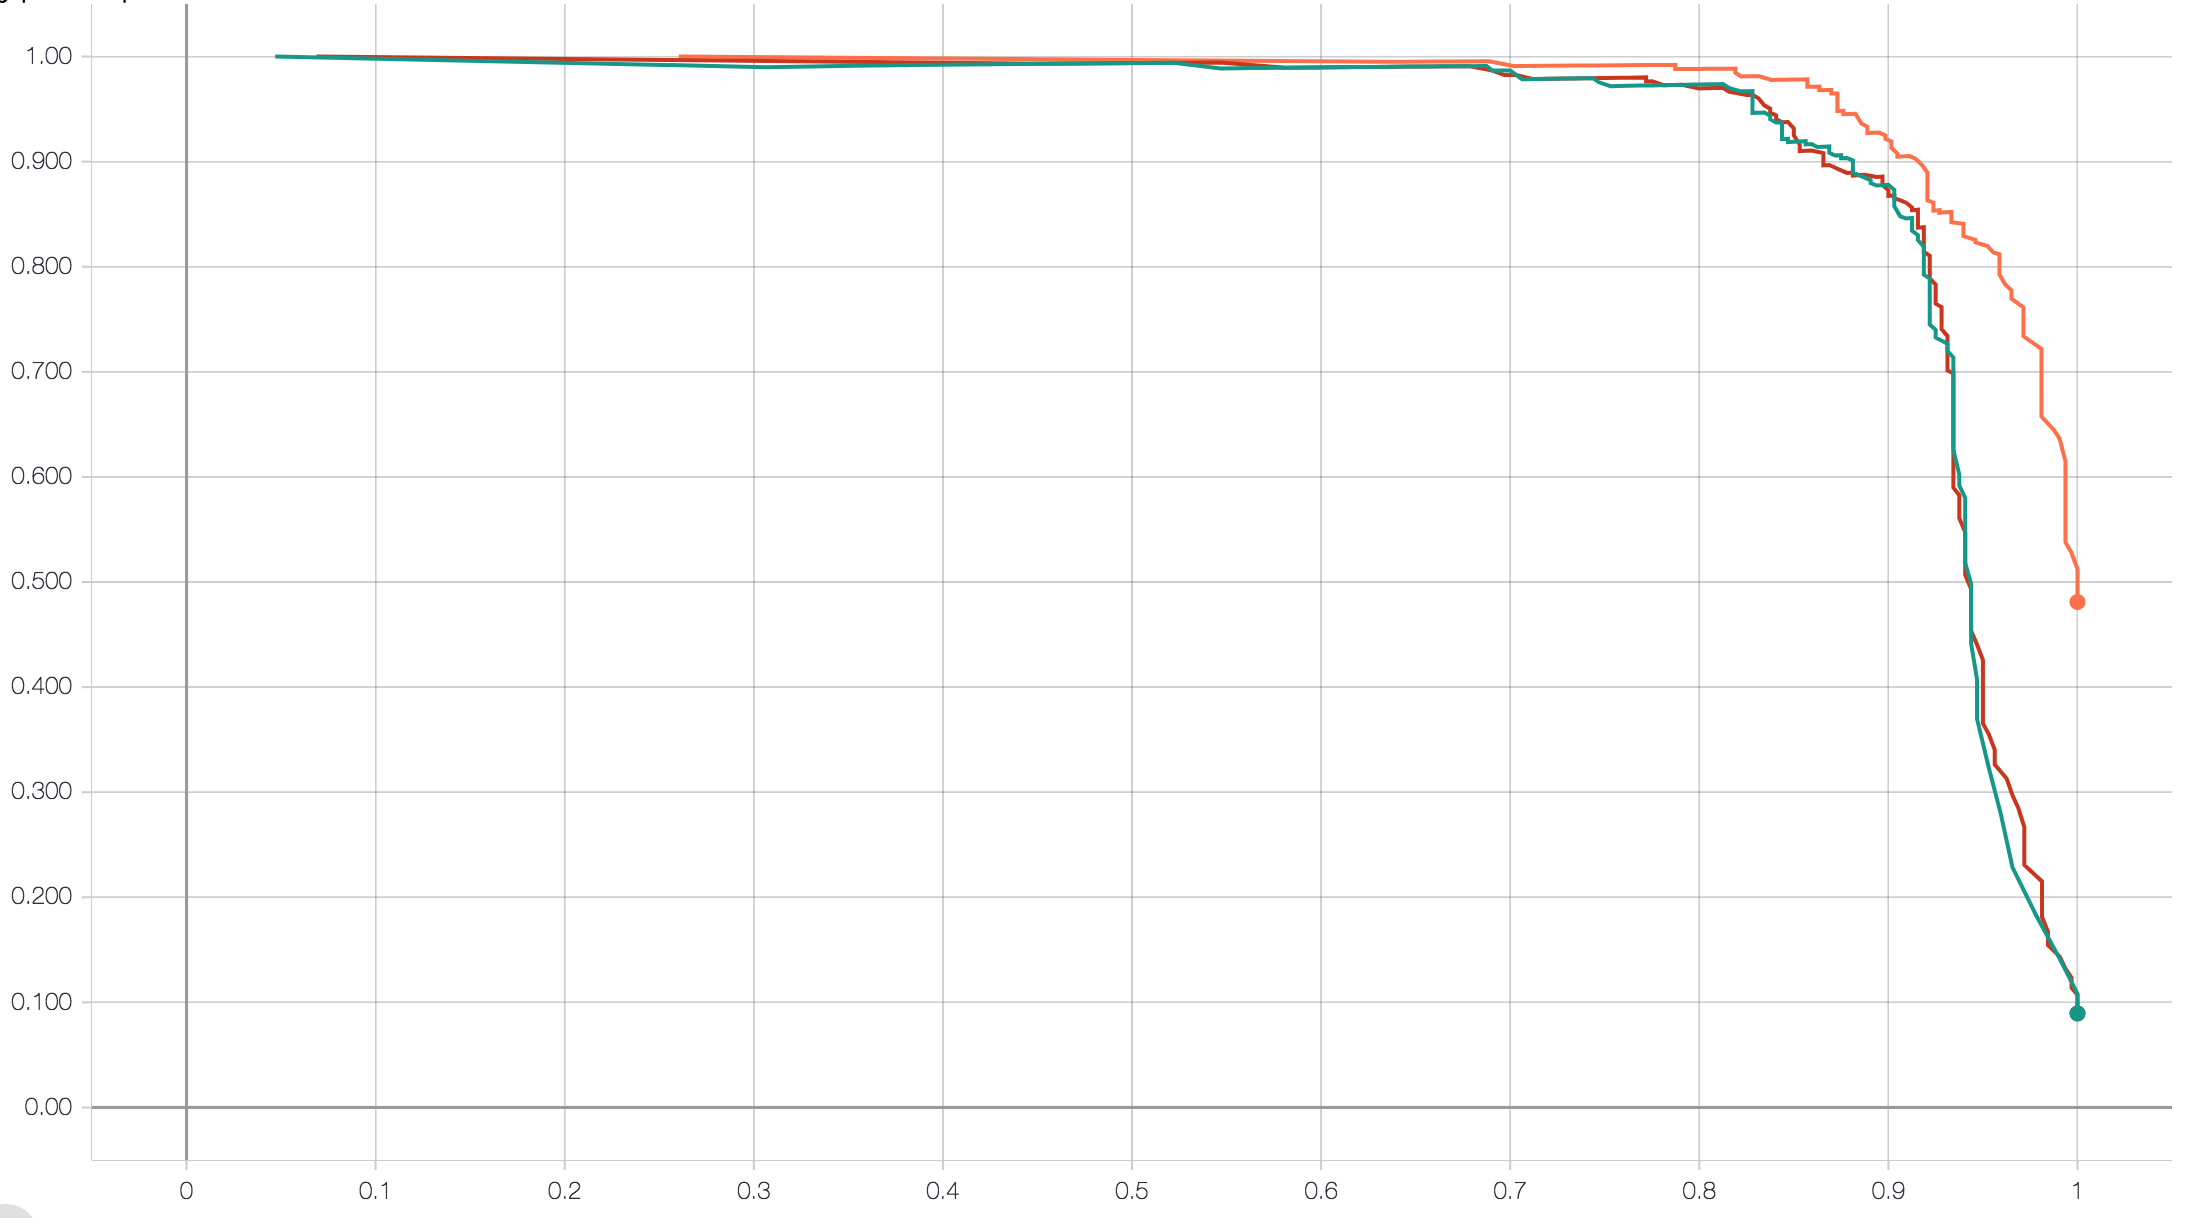
\includegraphics[scale=0.30]{img/precision-recall_curve_normal_undersampled_class_weights.png}
\caption{Precisão da classe positiva em função do \textit{Recall} da mesma classe, consoante o limiar de classificação das duas classes é alterado. Legenda: a verde o melhor modelo da experiência anterior (Secção~\ref{sec:optimizers}); a vermelho a experiência resultante da alteração dos pesos das classes (Tabela~\ref{tab:class_weights}); e a laranja a experiência resultante de \textit{undersampling} (Tabela~\ref{tab:undersampling}).}
\label{fig:precision-recall_curve_normal_undersampled_class_weights}
\end{figure}


%************************************************************************************
%************************************************************************************

\section{Conclusões}
\label{sec:conclusao}
 	Primeiramente, acreditamos que o nosso conhecimento sobre redes neuronais foi consideravelmente aprofundado, mostrando-se assim o grupo satisfeito com a escolha de tema realizada. De facto, Redes Neuronais artificiais representam uma abordagem a problemas bastante atuais, contribuindo assim ainda mais para o interesse do grupo no trabalho.
    
	É também evidente que Redes Neuronais artificiais se revelam uma ferramenta extremamente útil, apropriada para resolver problemas semelhantes ao apresentado, resultando numa abordagem ao problema bastante diferente de tudo aquilo com o que nós, como alunos do 3º ano de Informática, tínhamos tido a oportunidade de trabalhar.
    
	Após a primeira experiência, os resultados obtidos revelaram-se promissores sendo a precisão do melhor modelo \textit{97.93\%}. No entanto, o grupo considerava ser possível o melhoramento desse resultado, principalmente as métricas referentes à classe positiva, e optou por realizar um estudo exaustivo das possíveis abordagens e modificações que pudessem melhor o modelo utilizado. Da segunda experiência resultaram modelos evidentemente melhores em relação à classe positiva, com aumentos do \textit{F1-score} de 3 pontos percentuais no modelo treinado nos dados reamostrados (com frequência das classes rebalanceadas - \textit{undersampling}). A última experiência resultou em melhorias diminutas, sendo no entanto muito úteis para a nossa aprendizagem, e para um melhor entendimento do problema em causa.
	
	Em suma, concluimos que as experiências tiveram muito bons resultados, podendo ser útil o uso de \textit{undersampling} consoante o objetivo recaia mais na recolha de dados da classe positiva ou numa boa precisão global.

\section{Melhoramentos}
\label{sec:melhoramentos}
	Durante todo o trabalho fizemos uma pesquisa exaustiva da configuração da rede e dos seus hiper-parâmetros, o que nos leva a acreditar na qualidade dos nossos resultados.
    
    Mesmo assim poderemos ter alguns melhoramentos na pesquisa mais aprofundada de alguns hiper-parâmetros como a \textit{learning rate} do modelo (pesquisa por \textit{Grid Search}).
    
    Para além disso seria benéfico termos acesso a um maior \textit{dataset}, ou a um \textit{dataset} com melhor equilíbrio entre classes, dado que o \textit{dataset} usado no treino da nossa rede tinha uma vasta discrepância na quantidade de pulsares válidas.
    
    Estes melhoramentos levar-nos-iam a uma melhoria garantida do desempenho dos modelos.
    
\newpage

%************************************************************************************
%************************************************************************************

\section{Recursos}
\subsection{Bibliografia}

Abadi, Martín, Paul Barham, Jianmin Chen, Zhifeng Chen, Andy Davis, Jeffrey Dean, Matthieu Devin et al. "TensorFlow: A System for Large-Scale Machine Learning." In OSDI, vol. 16, pp. 265-283. 2016.
\\

Chollet, François. "Keras." KerasCN Documentation (2017): 55.
\\

Pedregosa, Fabian, Gaël Varoquaux, Alexandre Gramfort, Vincent Michel, Bertrand Thirion, Olivier Grisel, Mathieu Blondel et al. "Scikit-learn: Machine learning in Python." Journal of machine learning research 12, no. Oct (2011): 2825-2830.
Harvard	
\\

Lemaître, Guillaume, Fernando Nogueira, and Christos K. Aridas. "Imbalanced-learn: A python toolbox to tackle the curse of imbalanced datasets in machine learning." Journal of Machine Learning Research 18.17 (2017): 1-5.
\\

Lyon, Robert James. "Why are pulsars hard to find?." PhD diss., University of Manchester, 2016.
\\

R. J. Lyon, B. W. Stappers, S. Cooper, J. M. Brooke, J. D. Knowles, Fifty Years of Pulsar Candidate Selection: From simple filters to a new principled real-time classification approach, Monthly Notices of the Royal Astronomical Society 459 (1), 1104-1123, DOI: 10.1093/mnras/stw656
\\

Ruck, Dennis W., Steven K. Rogers, Matthew Kabrisky, Mark E. Oxley, and Bruce W. Suter. "The multilayer perceptron as an approximation to a Bayes optimal discriminant function." IEEE Transactions on Neural Networks 1, no. 4 (1990): 296-298.
\\

\subsection{Software}
\label{sec:software}
\begin{itemize}
  \item IDE: Visual Studio Code
  \item Linguagem de Programação: Python3
  \item Bibliotecas: Keras, Tensorflow, Scikit-learn, Imbalanced-learn
  \item Ferramentas: TensorBoard
\end{itemize}


\subsection{Divisão do Trabalho pelos Elementos do Grupo}
\begin{itemize}
  \item André Miguel Ferreira da Cruz: 36\% % actually 90% mas tasse
  \item Edgar Filipe Amorim Gomes Carneiro: 32\% 
  \item João Filipe Lopes de Carvalho: 32\%
\end{itemize}


\newpage

\appendix
\section{Appendix}
\label{sec:appendix}

\subsection{Manual do Utilizador}
\label{sec:manual}
\textbf{Instalar dependências:}
 \begin{enumerate}
  \item Abrir um novo terminal na raiz do projeto;
  \item Instalar todas as dependências, como descrito a baixo, executando o comando:
    \begin{lstlisting}
      pip3 install -r requirements.txt
    \end{lstlisting}
\end{enumerate}

\textbf{Executar através do terminal:}
\begin{enumerate}
	\item Abrir um novo terminal na pasta "./src" do projeto;
  	\item Executar o seguinte comando para treinar e avaliar o modelo:
    \begin{lstlisting}
		python3 main.py
	\end{lstlisting}
    
    \item Executar o seguinte comando para executar \textit{GridSearch} sobre uma rede de hiperparâmetros (referente à experiência da Secção~\ref{sec:tamanho_das_layers}):
    \begin{lstlisting}
		python3 grid_search.py
	\end{lstlisting}
    
\end{enumerate}
  
\textbf{Executar com interface \textit{Jupyter}:}
\begin{enumerate}
  \item Abrir um novo terminal na pasta do projeto;
  \item Executar o comando:
	\begin{lstlisting}
		jupyter notebook
	\end{lstlisting}
  \item Na \textit{Dashboard} do Jupyter, selecionar o projeto pretendido dentro da pasta "./src/notebook";
  \item Na nova janela aberta, carregar no botão \textit{Run};
  \item Por fim, esperar que a simulação acabe para visualizar os resultados.
\end{enumerate}
  	
\subsection{Dependências das Bibliotecas}
Para correr o código fornecido em anexo é necessário instalar as devidas dependências e bibliotecas. Para além das bibliotecas e ferramentas enumeradas na Secção~\ref{sec:software}, é necessário instalar as dependências usadas indiretamente. Para tal, e supondo que tem o python3 e o pip3 instalados, deve correr o seguinte comando a partir da raiz do projeto:
\begin{lstlisting}
pip3 install -r requirements.txt
\end{lstlisting}

Sendo o ficheiro \textit{requirements.txt} fornecido juntamente com o código, e tendo o seguinte conteúdo:

\begin{lstlisting}
absl-py==0.2.1
astor==0.6.2
bleach==1.5.0
gast==0.2.0
grpcio==1.12.0
h5py==2.7.1
html5lib==0.9999999
imbalanced-learn==0.3.3
imblearn==0.0
Keras==2.1.6
Markdown==2.6.11
numpy==1.14.3
protobuf==3.5.2.post1
PyYAML==3.12
scikit-learn==0.19.1
scipy==1.1.0
six==1.11.0
sklearn==0.0
tensorboard==1.8.0
tensorflow==1.5.0
tensorflow-tensorboard==1.5.1
termcolor==1.1.0
Werkzeug==0.14.1
\end{lstlisting}

\end{document}